\section{Introduction}

With the advent of Internet of Things, the evolution of mobile computing, and the emergence of real-time applications, the processing of an exponentially increasing volume of data must be performed in a timely fashion, i.e., with minimum latency. Despite the elasticity and vast computing power of existing cloud platforms, the access to these resources involves multiple hops of network communication, adding prohibitive latency to requests' processing. Such limitation has the following implications:

\begin{enumerate}

\item Cloud services may fail to satisfy the requirements of real-time and low-latency client applications; and

\item Offloading of delay-sensitive computation from devices with constrained resources to cloud servers is unlikely to work due to network-latency.

\end{enumerate}

\begin{figure}[htbp]
	\centering
	\subfloat[TODO: replace this image to avoid copyright problems.\label{fig:connected-vehicles}] {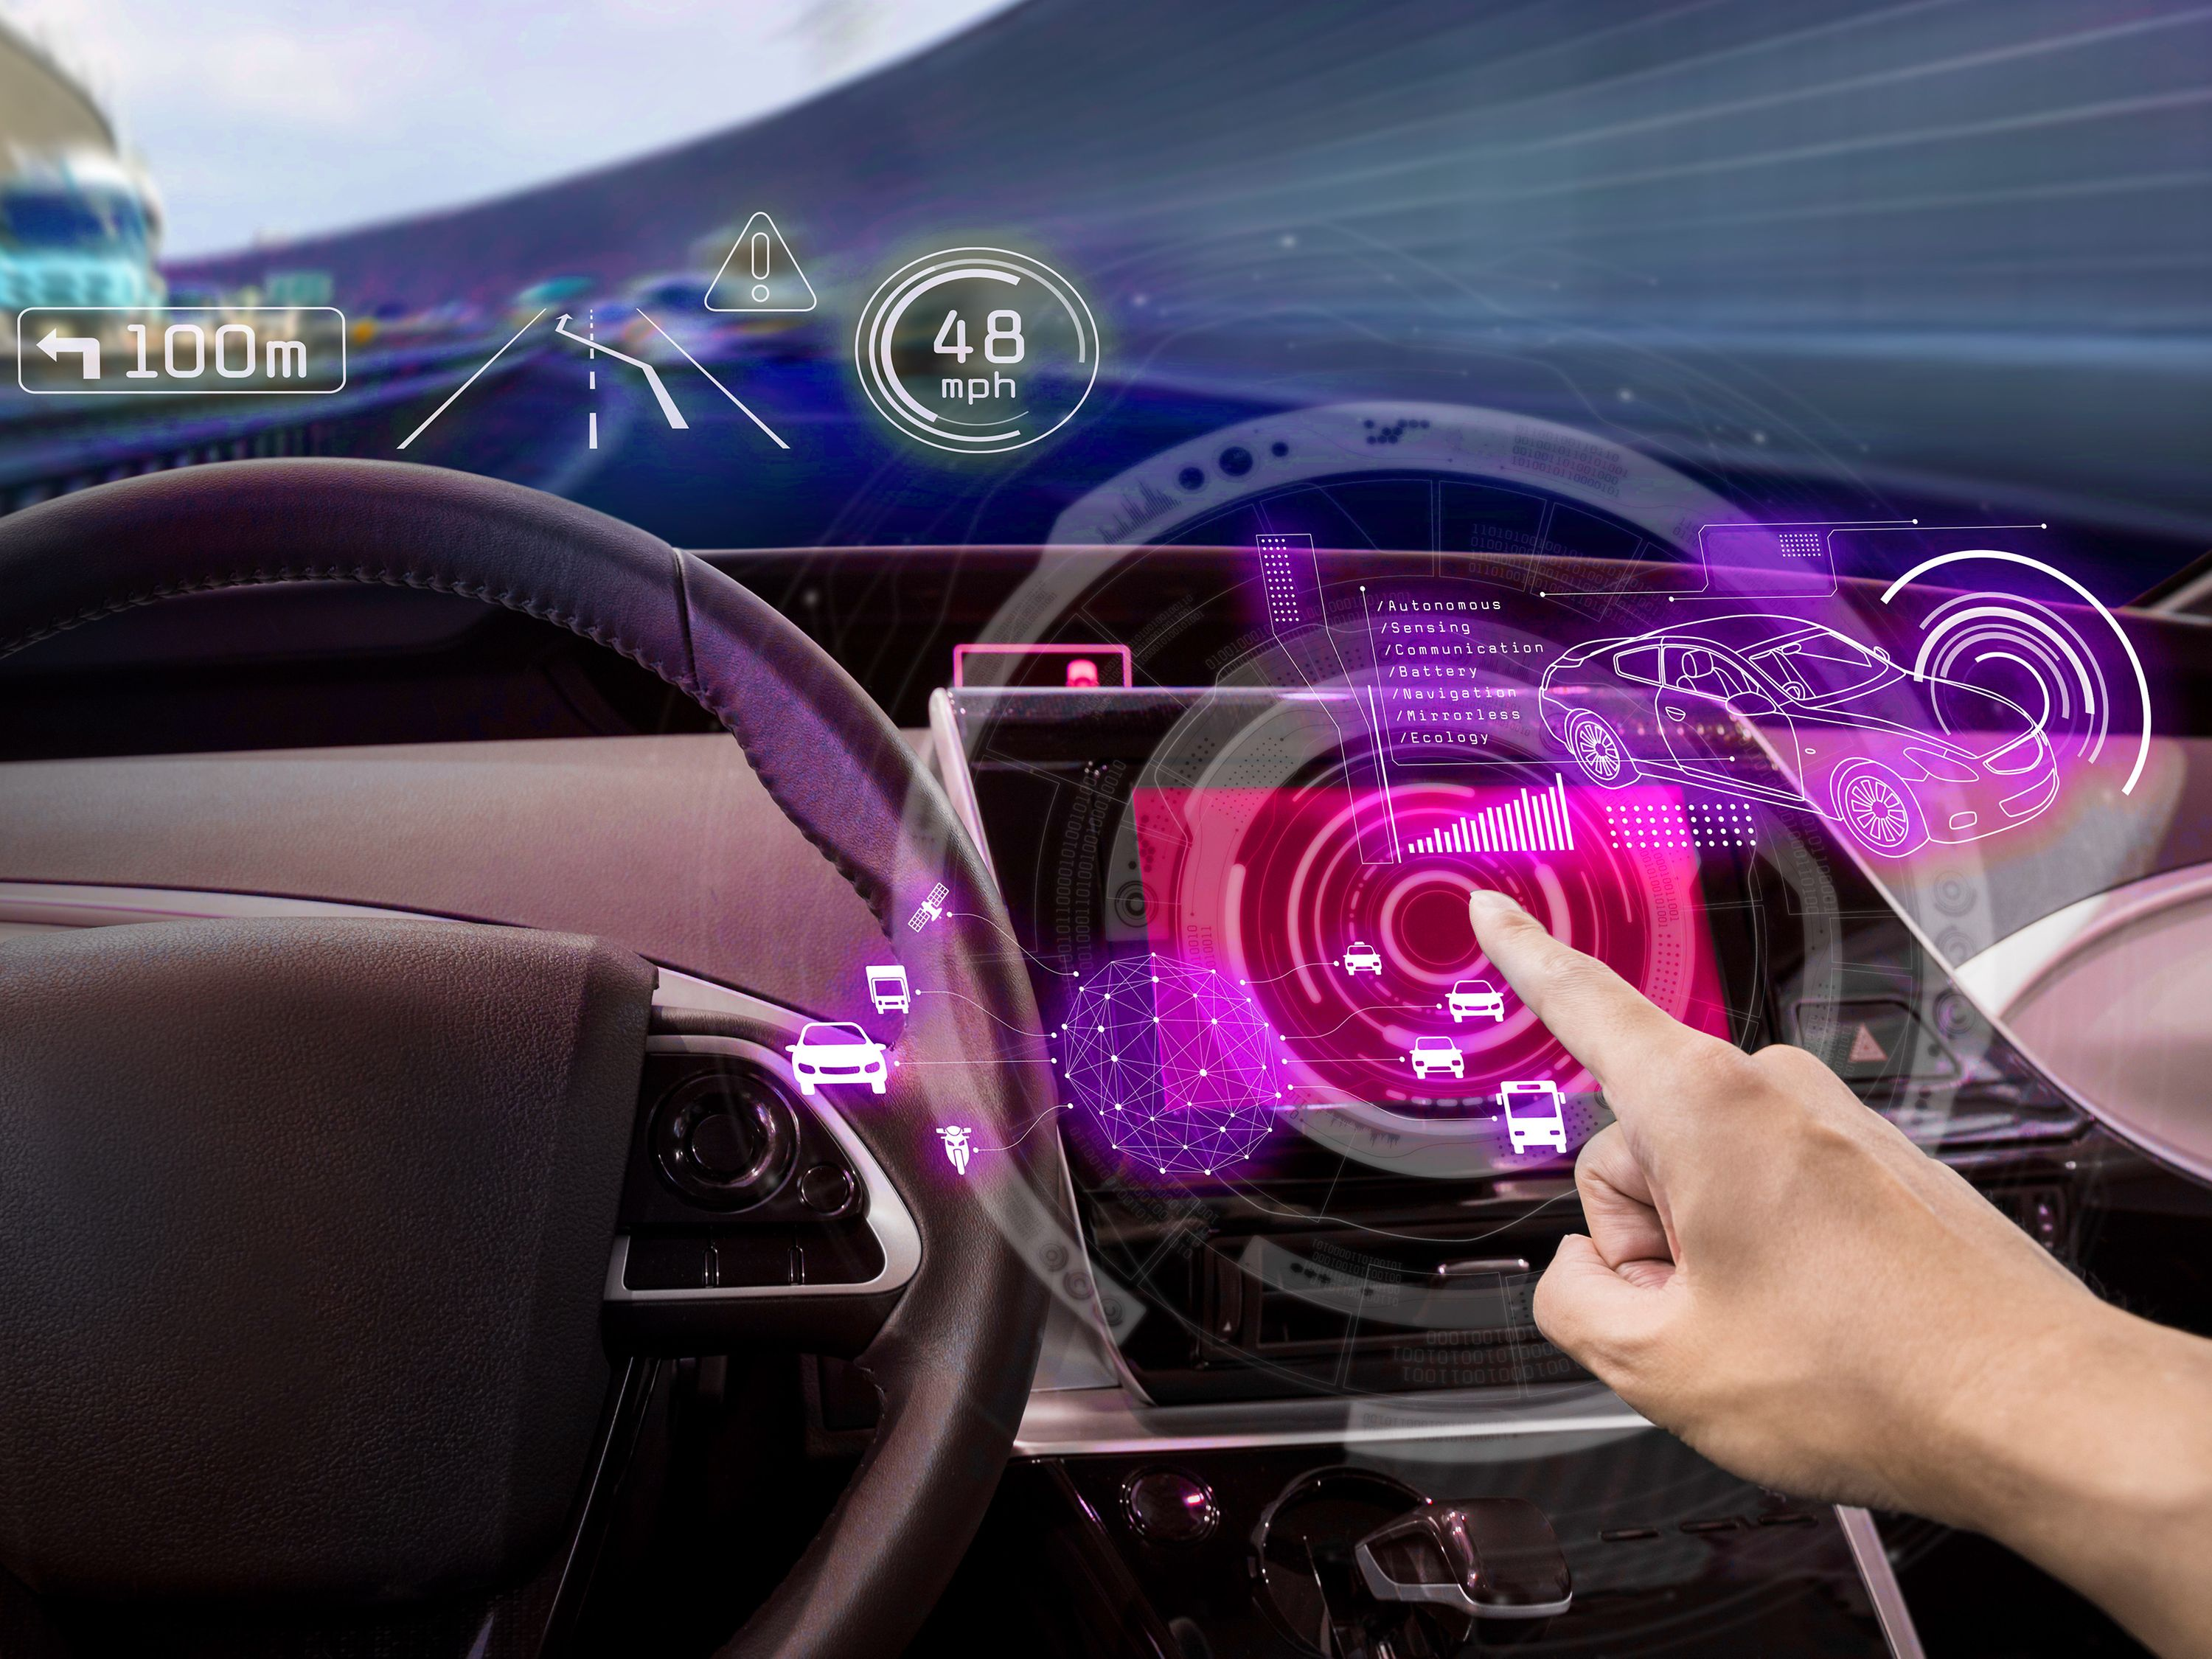
\includegraphics[width=0.47\textwidth]{figs/connected-vehicles.jpg}}\hfill
	~
	\subfloat[TODO: replace this with a less depressive image of augmented reality :)\label{fig:augmented-reality}]{
\includegraphics[width=0.53\textwidth]{figs/augmented-reality.jpg}}\hfill
	\caption{Different application types can be enabled or benefit from the low-latency of services deployed to nearby edge servers} \label{fig:motivational-cases}
\end{figure}

\subsection{Edge Computing}

To reduce network latency, data processing must be performed closer to where it is produced and consumed. In accordance with this principle, the emerging paradigm of edge computing~\cite{} states that computing power should be pushed from centralized datacenters to the edge of the network. The realization of this paradigm, however, still poses many challenges:

%
--- First, a highly distributed edge infrastructure is not expected to exhibit virtually unlimited resources as cloud datacenters. This limitation requires a more efficient allocation of edge resources. Current models based on virtualization and containerization, although successfully adopted by cloud providers, may not be feasible in the context of edge computing.

--- Second, cloud services cover very large areas in which requests from clients are always expected. In contrast, edge infrastructure features a fine-grained coverage area~\cite{Dehos14millimeter5g} where edge services would remain idle whenever clients are absent in their coverage area. Therefore, to optimize the usage of edge resources, edge infrastructure should support the opportunistic deployment of services.

%, accessible through well-known Internet names, edge services 

--- Third, different types of edge computing infrastructure may exist, including servers located at cellular base stations, temporarily placed nearby public events, and inside buildings and houses to provide support for smart environment applications. The eventual co-existence of edge alternatives would require the client-side participation on the decision of which alternative to use.

--- Finally, edge computing should complement rather than replace the cloud-based services. In this sense, edge computing should be seen as part of a continuum with the cloud in which opportunistic edge services are backed by cloud counterparts with high availability. Additionally, given the physical proximity between mobile clients and edge servers, the offloading of delay-sensitive computation from resource constrained devices to edge servers becomes possible. Also in this case, the opportunistic nature of edge services should be balanced with the high availability of local computation. Together, cloud, edge, and mobile should form what we call a \textit{computational continuum}.

%--- Last but not least, cloud servers should not be disregarded as a part of the Cloud-to-Edge continuum. %not sure whether to call it Cloud-to-Things or Cloud-to-Edge
%First, because client applications may still rely on Cloud backends for traditional, non delay-sensitive computation. Second, because edge servers may be unavailable from the certain locations. Thus, client applications must rely on a runtime mechanism to discover and negotiate the use of nearby edge infrastructure. As the alternative infrastructures (including the cloud) may exhibit uneven loads in different moments, the decision of which to use, must take into account their current status as well as the client application requirements in terms of latency and computational power. 


%Finally, to avoid increasing the burden of application development, computation to be executed at the edge should follow, to the extent possible, a common architecture and implementation with respect to its cloud counterpart. The same applies to the computation that may be offloaded from resource constrained devices to nearby edge infrastructure.  

\subsection{Serverless Computing}

Serverless computing~\cite{roberts2016serverless, hendrickson2016serverless}, also known as Functions-as-a-Service (FaaS)~\cite{mateosFaas17}, emerged as an alternative execution model within cloud computing. In particular, its name derives from the fact that server management and capacity planning decisions are hidden from the software application engineers. Instead, third party providers of the serverless platform dynamically manage the allocation of machine resources for the execution of different types of computational tasks, known as \textit{functions}. Today, multiple vendors provide serverless runtime and database services. 

Among its main advantages, the serverless model is considered to be cost- and resource-efficient in comparison to virtual machine and container-based provisioning models, which generally involve significant periods of underutilization or idle time. In previous work~\cite{GarrigaMendonca2017}, we discussed the suitability of a serverless architecture to enable low-latency applications to use edge computing computational resources in an efficient, scalable and automated way. Additionally, mobile devices could make use of compute runtimes deployed at nearby edge servers to extend their capabilities. Notwithstanding the potential of such combination, a complete model for its realization is still missing~\cite{NasticServerlessEdge17}. 

\subsection{Contributions of this Work}

In this work, we propose A3-E, a unified model for the computation continuum formed by mobile, edge, and cloud computational resources. The proposed model is aligned with the paradigm of serverless computing. In specific, A3-E explores the FaaS model to allow stateless computation to be quickly acquired, deployed, and made ready for execution. Due to its particular characteristics, which inherit and complement those of serverless computing, A3-E provides a suitable model for the realization of edge computing as part of a  computational continuum composed of cloud, edge, and mobile clients.

As has been demonstrated with experiments, client applications can rely on opportunistically selected services implemented as functions that are executable locally, in the edge, or in the cloud. Our experiments have shown a substantial reduction of latency when services are deployed to nearby edge infrastructure, as well as the battery consumption when computation is offloaded from mobile devices to edge or cloud servers.

%Last but not least, our contribution also includes a reference architecture for the realization of the proposed model. 

\subsection{Paper Organization}

The rest of this paper is organized as follows. Section~\ref{sec:motivation} describes the main motivation behind this work, including application scenarios and the computational continuum. Section~\ref{sec:background} provides a brief background on the main topics and concepts used by this work. Section~\ref{sec:proposal} provides a detailed description of the A3-E model. Section~\ref{sec:evaluation} reports on the experiments performed to evaluate our proposal with an augment reality application. Finally, Section~\ref{sec:conclusion} concludes this paper with our conclusions and future works.




